\documentclass[a4paper,10pt]{article}
\usepackage{anysize}
\usepackage{amsmath}
\usepackage{amssymb}
\usepackage{graphicx}
\usepackage[left=0.75in, right=0.75in, top=0.5in, bottom=0.75in, includefoot, headheight=13.6pt]{geometry}
\usepackage{color,graphicx}
\usepackage{verbatim}
\usepackage{hyperref}
\usepackage{multirow}
\usepackage{latexsym}
\usepackage{mdwlist}
\usepackage{tabularx}

\renewcommand{\labelitemii}{$\circ$}
% Education -> Internships -> Projects -> Tech Skills 
\hypersetup{
    bookmarks=true,         % show bookmarks bar?
    unicode=false,          % non-Latin characters in Acrobat's bookmarks
    pdftoolbar=true,        % show Acrobat's toolbar?
    pdfmenubar=true,        % show Acrobat's menu?
    pdffitwindow=true,      % page fit to window when opened
    pdftitle={CV},    % title
    pdfauthor={Gunjan},     % author
    pdfsubject={Placements},   % subject of the document
    colorlinks=true,       % false: boxed links; true: colored links
    linkcolor=magenta,        % color of internal links
    citecolor=blue,        % color of links to bibliography
    filecolor=magenta,      % color of file links
    urlcolor=black           % color of external links
}

% Margines

\addtolength{\oddsidemargin}{-0.215in}
\addtolength{\textwidth}{0.2in}

\definecolor{titleColor}{rgb}{0.631, 0.776, 0.925}

\begin{document}

%%%%%%%%% virtical space %%%%%%%%%%%%%%%%%


\begin{table}[h!]
  \begin{center}
    \begin{tabular}{  l  p{10cm}  p{8cm}}
      \raisebox{-\totalheight}{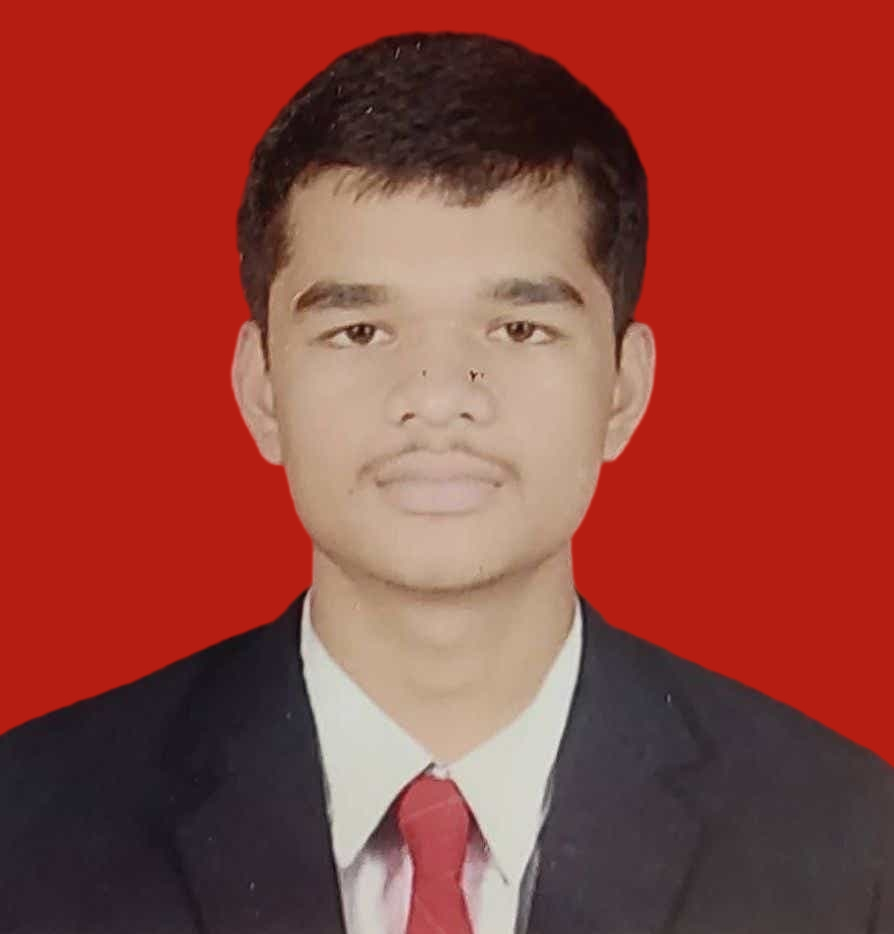
\includegraphics[scale=.075]{gunjan}}
       &
      \begin{itemize}
        \setlength\itemsep{.01em}
        \item[] \textbf{Gunjan Atul Lunkad}
        \item[] \textbf{\href{mailto:glunkad26@gmail.com}{glunkad26@gmail.com}}
        \item[] \textbf{\url{http://www.linkedin.com/in/gl-gunjan-lunkad}}
        \item[] \textbf{\url{http://github.com/glunkad}}
      \end{itemize}
       &
      \begin{itemize}
        \setlength\itemsep{.01em}
        \item[] \textbf{Male}
        \item[] \textbf{DOB: 26/01/2001}
        \item[] \textbf{+91 7620980424}
      \end{itemize}
    \end{tabular}
  \end{center}
\end{table}

\vspace{-.8cm}

\begin{tabularx}{.98\textwidth}{llp{2cm}lll}
  \hline
  \textbf{Examination} & \textbf{Specialization}          &  & \textbf{University / Board} & \textbf{Year} & \textbf{CPI} \\
  \hline
  Graduation           & Electronics \& Telecommunication &  & PCCOE                       & 2023          & 8.82/10      \\
  Intermediate         & -                                &  & HSC                         & 2019          & 69.8/100     \\
  Matriculation        & -                                &  & SSC                         & 2017          & 87.6/100     \\
  \hline
\end{tabularx}
\\\\

\colorbox{titleColor}{\parbox{6.7in}{\textbf{WORK EXPERIENCE}}}

\begin{itemize*}
  \setlength{\itemsep}{.00pt}
  \item \textbf{{PyNote: Open Source}} \hfill {\small{{\textbf{[June 2023]}}\/}}
  \begin{itemize*}
    \item \textbf{Enhanced PyNote}.\\
    Engineered the "Control+S" functionality, elevating the file-saving process in the PyNote text editor application written in Python and Tkinter.
  \end{itemize*}
\end{itemize*}

\begin{itemize*}
  \setlength{\itemsep}{.00pt}
  \item \textbf{{AppFlowy: Open Source}} \hfill {\small{{\textbf{[Feb 2023]}}\/}}
  \begin{itemize*}
    \item \textbf{Engineered AppFlowy Parsing}.\\
    Developed a code block parser in Flutter for AppFlowy, introducing a structured approach to code presentation.
  \end{itemize*}
\end{itemize*}

\colorbox{titleColor}{\parbox{6.7in}{\textbf{ PROJECTS}}}


\begin{itemize*}
  \setlength{\itemsep}{1pt}
  \item \textbf{\small{Phonebook}} \hfill {\small{{\textbf{[May 2023]}}}\/}
  \begin{itemize*}
    \item Developed and refined a React-based phonebook application, allowing users to add and filter contacts.
    \item Enhanced user experience by preventing duplicate entries, issuing alerts for existing contacts, and implementing backend communication for data storage and retrieval.
  \end{itemize*}
\end{itemize*}

\begin{itemize*}
  \setlength{\itemsep}{1pt}
  \item \textbf{\small{Countries data}} \hfill {\small{{\textbf{[Jan 2023]}}}\/}
  \begin{itemize*}
    \item Created a user-friendly Vite.js web application, refining the search interface and dynamically displaying country details.
  \end{itemize*}
  \begin{itemize*}
    \item Revamped the application by seamlessly integrating weather data from https://openweathermap.org/, while instituting secure API key management through environment variables.
    features such as user authentication, email-based user verification, and password reset functionality.
  \end{itemize*}
\end{itemize*}

\begin{itemize*}
  \setlength{\itemsep}{1pt}
  \item \textbf{\small{Strawberry Stacker}} \hfill {\small{{\textbf{[Nov 2022]}}}\/}
  \begin{itemize*}
    \item     Engineered the Strawberry Stacker project, creating an innovative algorithm that enables the remote control of drones through a web application integrated with various APIs.
    \item Instituted a seamless interaction between the web app and drones, showcasing proficiency in algorithmic development and API integration.
  \end{itemize*}
\end{itemize*}

\colorbox{titleColor}{\parbox{6.7in}{\textbf{TECHNICAL SKILLS}}}\\

\begin{tabular}{p{1.6in}p{0.1in}p{4.5in}}
  \textbf{\small{Programming Languages}} & : & {{Python, JavaScript}}  \\
  \textbf{\small{Web Technologies}}      & : & {{React, Django}}       \\
  \textbf{\small{Database}}              & : & {{MongoDB}}             \\
  \textbf{\small{Version Control}}       & : & {{Git, Github}}         \\
  \textbf{\small{Softwares/Tools}}       & : & {{ Visual Studio Code}} \\
\end{tabular}



%\begin{itemize*}
%  \setlength{\itemsep}{1pt}
%  \item \textbf{\small{M.Tech Seminar: Review of Methods of Speech Synthesis}} \hfill {\small{{\textbf{[Jun '11 - Nov '11]}}}\/} 
%\begin{itemize*}
%	\item Speech synthesis is the technique of converting given input text to synthetic speech.
%	\item A comprehensive literature review of majorly researched methods of speech synthesis was done.
%\end{itemize*}
%\end{itemize*}

%\begin{itemize*}
%  \setlength{\itemsep}{1pt}
%  \item \textbf{\small{An aid in communication for the mute}} \hfill {\small{{\textbf{[Aug '12 - Jan '13]}}}\/} 
%\begin{itemize*}
%	\item Project proposal selected for Texas Instruments(TI) analog design contest 2012.
%	\item Going to design a portable unit for the mute person which generates speech equivalent of his hand gestures.
%	\item Right now, we are working upon the 1st part of analog design contest i.e., simulation of 2nd order LPF using TL082
%         op-amp.
%\end{itemize*}
%\end{itemize*}

%\begin{itemize*}
%  \setlength{\itemsep}{1pt}
%  \item \textbf{\small{Discrete Logarithm Problem}} \hfill {\small{{\textbf{[Jan '12 -  May '13]}}}\/} 
%\begin{itemize*}
%	\item Implemented the BSGS method for solving DL problem for an extension field of prime 3 i.e., $3^m$ in SAGE.
%	\item Value is found upto 8 digits of input, and m is varied from 1 to 25.
%\end{itemize*}
%\end{itemize*}

\colorbox{titleColor}{\parbox{6.7in}{\textbf{Positions of Responsibility}}}\\

\textbf{Student Internship Co-ordinator, ECE Department}  \hfill {\small{{\textbf{[Sep 2020 - April 2023]}}}\/}
\begin{itemize*}
  \item Updated and maintained internship databases, ensuring accurate and up-to-date records of student placements, achievements, and feedback.
  \item Provided guidance and support to students throughout their internship journey, addressing concerns, and fostering a positive and enriching learning environment.
\end{itemize*}

%\textbf{PG Coordinator, Robotics Club, STAB} \hfill {\small{{\textbf{[Jul '12 - Apr '13]}}}\/} 
%\begin{itemize*}
% \item Responsible for increasing PG participation in institute level technical activities.
%% \item Organised ROFL (Research Only for Fun) event for PG students.
% \item Selected as the Best PG Coordinator for my contribution to the club.
%\end{itemize*}

%\textbf{Techical Secretary, H14, IIT Bombay} \hfill {\small{{\textbf{[Jul '12 - Apr '13]}}}\/} 
%\begin{itemize*}
% \item Ensured adequate hostel representation in institute level technical activities.
%\end{itemize*}

%\textbf{Committee Head, Certificate and Memento, Confluence'08, NIT Kurushetra} 
%\begin{itemize*}
% \item Managed the preparation and distribtution of certificates and mementos in Confluence'08.
%\end{itemize*}


\textit{Updated on 17th Nov 2023}
\end{document}

